\chapter{Prototype}
\label{Chapter3}

In this chapter, we implement a prototype based on PTAM \cite{Reference12}. The prototype integrates the five methods in section \ref{VisualizationMethods}. It provides realtime video with no requirement for any GPS or gyrocompass devices. A use case is in section \ref{UseCases}.

%------------------------------------------------------------------------------

\section{System Architecture}

The mobile device used in the prototype is a Sony VAIO VGN-UX90PS (see appendix \ref{AppendixA}). We base our program on the PTAM reference implementation source code \cite{Reference16} to get the position and orientation of the VAIO. However, this implementation cannot run on the VAIO because it requires a dualcore CPU computer to be able to run smoothly. As a result, we connect a MacBook Pro (appendix \ref{AppendixB}) to the VAIO and the PTAM part of the program will run on the MacBook (figure \ref{fig:VAIOMacBookPro}).

The programs on both VAIO and MacBook Pro run on Microsoft Windows XP SP2 operating system. For the sake of quick setup time, the VAIO and the MacBook are connected directly using ad hoc mode, which means that an additional wireless hub is not needed. The VAIO and the MacBook are connected by a 11Mbps wireless network. The network interfaces on both VAIO and MacBook Pro are able to work at 54Mbps, but for some reason of Windows they can only work at 11Mbps. This is an unexpected problem which lowers the speed, and consequently the accuracy and stability of the prototype system. We can also use LAN cable for even faster 100 Mbps speed, but the VAIO will be wired to another bulky device, which is not desirable because the mobility of the VAIO is totally lost.

%------------------------------------------------------------------------------

\section{Server-side PTAM}

We modify the original PTAM source code so that the ``video source'' is remotely located on the VAIO, not on the MacBook. We learn a little from Erlang language \cite{Reference17} of how to write concurrent, high-performance systems. Right after the TCP (Transmission Control Protocol) connection between the VAIO and the MackBook is established:

\begin{itemize}
	\item The VAIO continuously feeds frames captured from its camera to the MacBook.
	\item The MacBook continuously feeds position and orientation of the camera of the VAIO to the VAIO.
\end{itemize}

As the above explanation suggests, we use ``push'' instead of ``pull'', one side actively sends data to the other side without having to wait for the request for the data from the other side. In other words we use the mailbox design pattern instead of the RPC (Remote Procedure Call) design pattern, which is slower and requires synchronizing the call and the result (figure \ref{fig:MailboxRPC}).

\begin{figure}[htbp]
	\centering
	\includegraphics{./Figures/mailbox_rpc.png}
	\rule{35em}{0.5pt}
	\caption[Mailbox vs. RPC]{Mailbox (above) vs. RPC (below)}
	\label{fig:MailboxRPC}
\end{figure}

Because PTAM only need grayscale frames, instead of sending all the three RGB color channels of the frames, the VAIO only need to send the brightness Y = 0.3*R + 0.59*G + 0.11*B. There are several optimizations to further improve the frame rate sent to the MacBook:

\begin{itemize}
	\item Send G color channel instead of Y, because G affects Y the most as in the above common equation. This does not affect PTAM. This optimization enormously improves the frame rate because when we send Y, if the image size is 320x240, we must apply the above equation 76800 times for each frame!
	\item Losslessly compress G color channel using the standard library ``zlib''. The compression rate is about 50\%.
\end{itemize}

\begin{table}[tb]
	\begin{center}
		\caption{Frame rates of various conditions}
		\label{tb:FrameRates}
		\begin{tabular}{|c|c|c|r|}
			\hline
			Size (only green color channel) & Compressed & With PTAM processing & FPS   \\
			\hline
			320x240 & NO         & NO                   &  8.01 \\
			320x240 & YES        & NO                   & 10.67 \\
			640x480 & NO         & NO                   &  1.97 \\
			640x480 & YES        & NO                   &  3.03 \\
			320x240 & NO         & YES                  &  6.57 \\
			320x240 & YES        & YES                  &  6.23 \\
			640x480 & NO         & YES                  &  1.84 \\
			640x480 & YES        & YES                  &  1.69 \\
			\hline
		\end{tabular}
	\end{center}
\end{table}

However, as table \ref{tb:FrameRates} suggests, we should use 320x240 frame size with uncompressed green color channel. This gives smooth frame rate with be above system architecture and optimizations. Bigger frame size allows PTAM to find more feature points, but the following drawbacks pop up:

\begin{itemize}
	\item Data for each frame gets bigger. This increases data transmission time for each frame.
	\item The MacBook must process more data. This decreases the result frame rate.
\end{itemize}

When increasing from 320x240 to 640x480, the frame rate drop about 4 times, and the prototype no longer works smoothly as required in \ref{VisualizationRequirements}.

%------------------------------------------------------------------------------

\section{Pre-registered 3D Model and Viewing Field Visualization}
\label{3DModel}

On the VAIO, there is pre-registered positions and orientations of surveillance cameras. Having the position and orientation of itself tracked and fed by the MacBook, the VAIO can create CG objects and correctly overlay them on the screen to visualize the viewing fields.

To make the CG objects look more ``real'', we may also use a rough 3D model of the surrounding buildings. For example, in animation visualization method, we can stop the grid when it touch the surface of the building walls. The 3D model only contains planes, texture is not necessary.

%------------------------------------------------------------------------------

\section{Map Initializing and 3D Model Registering}
\label{MapInitializing}

PTAM continuously builds and maintains a 3D map by adding stable feature points and removing unstable ones taken from the frames (figure \ref{fig:Map}). The problem is the 3D model must be in match with this map. When the scene is unchanged, the map may be rotated or translated but relative positions among the feature points are preserved. Thus we have the following workflow:

\begin{enumerate}
	\item Initialization and registration phase: Let PTAM build the map. Manually translate and rotate the model to match the map (or vice versa), the save the translation and rotation parameters.
	\item Usage phase: On next program startups, as long as we can make sure that the map is not different from the map used to save the parameters, we can use the parameters to translate and rotate the model to match map.
\end{enumerate}

The reference implementation of PTAM initializes the map on each program startup by taking two keyframes which form a stereo pair (figure \ref{fig:Stereo}). As a result, there are two approaches to solve the map-model matching problem:

\begin{itemize}
	\item Control the two keyframes. This approach is easy because we simply take two images before-hand, then feed them to PTAM on each program startup. The scene in the two images is usually a scene of buildings. It is called a landmark. In the usage phase, PTAM allows the user at startup to stand at a slightly different position other than the ones where we took the two images (figure \ref{fig:Stereo}). This is convenient because normally it is very hard to return to the exact position after some time.
	\item In the initialization and registration phase, serialize the map to string and save the string to disk, then on usage phase just skip the map initialization, load the map from disk, deserialize and feed it directly to PTAM. We can prebuild a large fine-grain map to use in the usage phase, thus the system becomes very robust. Moreover, in the usage phase at startup the user can stand at a very different position and orientation, as long as the position is inside the prebuilt map.
\end{itemize}

The landmark can be thought as an ``access point'' as in wireless network terminology. Its appearance should not change too much over time so that it is usable. The second approach is in general more powerful than the first one, but if the scene changes too much then it may be less powerful because parts of the prebuilt map will become invalid and cause noise or heavy load to PTAM. The first approach always works given a good landmark, because the map can be updated dynamically by PTAM.

With the first approach, because of the reference implementation of PTAM requirement to make the map initialization stable, actually we must take about 5-10 images and feed them to PTAM, with the first and the last one act as the two keyframe (figure \ref{fig:2KeyFrames}). The video retrieving part and feature point processing part of PTAM run in two separate threads, as a result slightly different maps may be initialized each time PTAM during startup. To make sure that PTAM always initialize the same map, we must feed each frame for an enough amount time, about more than one second for the MacBook we are using.

\begin{figure}[htbp]
	\centering
	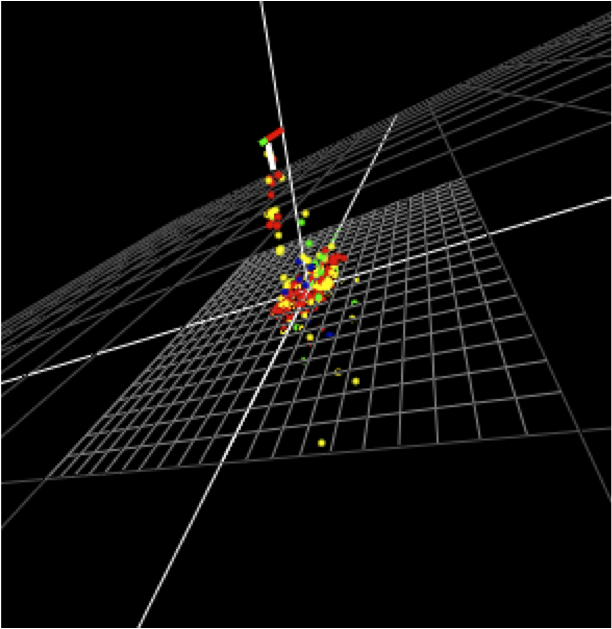
\includegraphics{./Primitives/map.png}
	\rule{35em}{0.5pt}
	\caption[Map]{Map}
	\label{fig:Map}
\end{figure}

\begin{figure}[htbp]
	\centering
	\includegraphics{./Figures/stereo.png}
	\rule{35em}{0.5pt}
	\caption[Map initialization]{Map initialization}
	\label{fig:Stereo}
\end{figure}

\begin{figure}[htbp]
	\centering
	\includegraphics{./Figures/2keyframes.png}
	\rule{35em}{0.5pt}
	\caption[Feeding frame to PTAM to initialize map]{Feeding frame to PTAM to initialize map}
	\label{fig:2KeyFrames}
\end{figure}

%------------------------------------------------------------------------------

\section{History of current prototype}

The prototype described in the above sections is not the only decision choice we have made throughout this research. Previously, we have made others as described below.

\subsection{Hardware -- Prototype with GPS and gyrocompass devices}

We have implemented a prototype with the architecture in figure \ref{fig:VAIOGPSGyro}. The GPS device specifications is in appendix \ref{AppendixD}. The GSP and gyrocompass devices provide position and orientation information of the mobile device. Together with the prebuilt CG information, we can overlay CG objects to visualize viewing fields of surveillance cameras. The update rate of the gyrocompass is 180Hz, which is high thus the orientation information is quite good. However, the GPS device error is about 5-10 m (figure \ref{fig:GPSError}), which affects badly the accuracy of the visualization. To improve the GPS device error, model-based tracking method as described in \cite{Reference13} method may be used.

\begin{figure}[htbp]
	\centering
	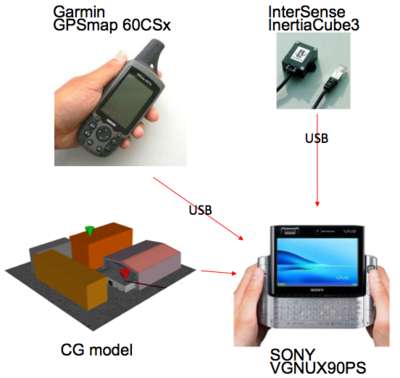
\includegraphics{./Primitives/vaio_gps_gyro.png}
	\rule{35em}{0.5pt}
	\caption[Prototype with GPS and gyrocompass devices]{Prototype with Sony VAIO VGN-UX90PS, Garmin GPSmap 60CSx, and InterSense InertiaCube3}
	\label{fig:VAIOGPSGyro}
\end{figure}

\begin{figure}[htbp]
	\centering
	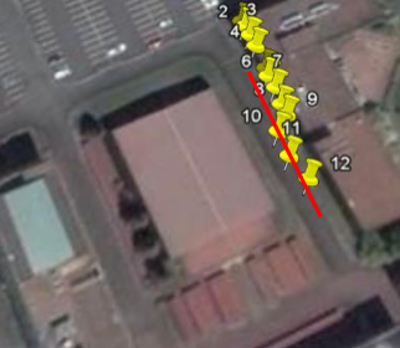
\includegraphics{./Primitives/gps_error.png}
	\rule{35em}{0.5pt}
	\caption[GPS error]{The points do not lie on the red line because of GPS error}
	\label{fig:GPSError}
\end{figure}

In the above prototype, we do not use GPS and gyrocompass devices. Although the more auxiliary devices we add the bulkier and more complicated in programming the mobile device becomes, GPS and gyrocompass devices can be used together with PTAM in the multi-sensor fusion \cite{Reference14} style, which may greatly improves the robustness of the system:

\begin{itemize}
	\item Initialization problem: the GPS and gyrocompass devices may provide initial position and orientation of the mobile device. Although the error of the GPS device is not small, in a large map it may help PTAM to reduce the search space.
	\item Quick movement: PTAM is image-based, thus it does not work well when the user quickly moves the mobile device. At this time, the gyrocompass may provide PTAM the orientation information because its update rate is high. Although the gyrocompass suffers from drifting error and needs to be continuously adjusted by the other sensors in the fusion, quick mobile device movement usually lasts only in a short time, thus gyrocompass may provide precious temporary information during this time.
\end{itemize}

\subsection{Software -- Development environment}

Visualization methods are expected to be found experimentally and visually. Thus, trial and error methodology is applied here. To shorten the trial and error cycle, we need a good development environment which allows quick compiling, running and modifying.

At first we used C/C++ language and OpenGL API \cite{Reference10}. Because both the language and the API are in too low level, the development speed was slow. Later, C/C++ language was fully replaced by Ruby language. Ruby is an object oriented strongly-typed dynamic language that attracts attention of developers world-wide in recent years. From the perspective of software engineering, the above features provide the following benefits:

\begin{itemize}
	\item Object oriented feature: Easy to structure the program and later maintain the source code over time.
	\item Strongly-typed feature: Variables have types, thus we can avoid bugs which usually occur in weakly-typed languages like PHP.
	\item Dynamic feature: There is no compile time. With static languages like C/C++, a lot time is wasted on compiling source code. With Ruby we can modify source code and run right away.
\end{itemize}

The development speed was better but still slow, partly because of the slow. It was concluded that the speed of the development is largely affected by the API rather than the language. Consequently, a higher level 3D rendering engine has been adopted: Irrlicht. Later, we read many reviews on the Internet that say that OGRE \cite{Reference11} is easier to use than Irrlicht, thus we migrated to OGRE. OGRE, Object-Oriented Graphics Rendering Engine, is a scene-oriented, flexible 3D rendering engine written in C++ designed to make it easier and more intuitive for developers to produce applications utilizing hardware-accelerated 3D graphics. The class library abstracts all the details of using the underlying system libraries like Direct3D and OpenGL and provides an interface based on world objects and other intuitive classes.

However, OGRE is generally used for creating 3D games thus contain too many features that we do not need. The framework forced us to write too much bloated code for the purpose of this research. As a result, we finally migrated to a combination of Ruby and C language with pure OpenGL API. At this time Ruby has grown to version 1.9. In this version the interpreter is replaced by a virtual machine, which boosts our Ruby program's speed to about 10x. Moreover importantly it is ridiculously easy to write C extension for Ruby \cite{Reference15}. For program parts that need speed like networking and image processing, we use the Ruby standard library which is written in C, or write them as C extension for Ruby. For program parts that need trial-error or does not need speed like the user interface part, we write them in pure Ruby.

In short, our experience suggests that keeping a balance between dynamic language and static language is a good choice.

%------------------------------------------------------------------------------

\section{Viewing Modes}

It is easier to understand a thing when we put it in a context. In real scene, users see the big picture of the area around them. Consequently, if we let the users see the map of the area where they are standing, the map will help them understand the visualized view fields of the surrounding surveillance cameras easier.

Because there is the 3D model on the VAIO as described in section \ref{3DModel}, we propose three viewing modes:

\begin{itemize}
	\item Camera mode: This is the mode mentioned in earlier chapters and sections. In this mode the frames taken by the VAIO's camera are overlaid with CG objects.
	\item Map mode: Map of the area of the current position is displayed on screen (figure \ref{fig:MapMode}).
	\item FPS (first-person shooter) mode: The users can navigate the 3D world as in FPS games. Using this mode, the users can virtually walk to other positions of the area to see viewing fields of surveillance camera at those positions.
\end{itemize}

\begin{figure}[htbp]
	\centering
	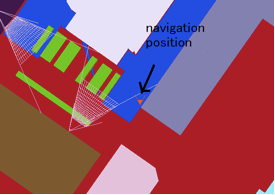
\includegraphics{./Primitives/map_mode.png}
	\rule{35em}{0.5pt}
	\caption[Map mode]{Map mode}
	\label{fig:MapMode}
\end{figure}

Keypads on mobile devices are usually hard to use, especially when the users use only one hand to both hold the device and press the keys. When a mobile device is equipped with a accelerometer (most cell phones today have one built-in) or gyrocompass, these auxiliary devices can be used for navigating around easier, existing applications of joysticks and iPhone have proved this. For example, in map mode the three degree-of-freedom variables of the gyrocompass can be used as in table \ref{tb:GyrocompassNavigation}):

\begin{table}[tb]
	\begin{center}
		\caption{Using gyrocompass for navigation}
		\label{tb:GyrocompassNavigation}
		\begin{tabular}{|c|l|l|}
			\hline
			Degree-of-freedom variable & Usage                     \\
			\hline
			Yaw                        & 360$^\circ$ rotation      \\
			Pitch                      & Forward-backward movement \\
			Roll                       & In/out zooming            \\
			\hline
		\end{tabular}
	\end{center}
\end{table}

\begin{figure}[htbp]
	\centering
	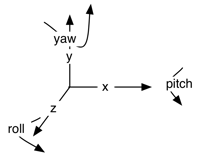
\includegraphics{./Primitives/yaw_pitch_roll.png}
	\rule{35em}{0.5pt}
	\caption[The three degree-of-freedom variables of a gyrocompass]{The three degree-of-freedom variables of a gyrocompass}
	\label{fig:YawPitchRoll}
\end{figure}
